\chapter{Linking Financialization and Urban Productivity} \label{chapter-tramsmission} %{Distribution and Growth} \label{chapter-distribution} % \chapter{Productivity Spillovers}  % \label{chapter-productivity-spillovers}

\epigraph{Alternative micro-foundations cannot be regarded as interchangeable contents for the black box \dots %The micro-foundations of urban agglomeration economies interact with other building blocks of urban models in ways that we cannot recognise unless they are explicitly stated. For instance, the composition of cities typically emerges as a consequence of the scope of different sources of agglomeration economies and their interaction with other aspects of individual behaviour. Third, 
different micro-foundations have different welfare and policy implications. %If we begin building an urban model by postulating an aggregate production function with increasing returns, we can only take this function as given. If instead we derive this aggregate production function from first principles, we may see that its efficiency can be improved upon. The means for achieving such an improvement will depend on the specifics of individual behaviour and technology. Thus, while different assumptions regarding individual behaviour and technology may support similar aggregate outcomes, the normative implications of alternative micro-foundations can differ substantially.
}{Duranton and Puga \cite{durantonMicroFoundationsUrbanAgglomeration2004}}

\epigraph{A large body of literature documents the existence of agglomeration economies in developed economies ... The main conclusion of this literature is the finding of scale economies of 3--8 percent (that is, a 10 percent increase in the size of an activity in a city raises productivity in this activity by 0.3--0.8 percent).}{Gilles Duranton \cite{durantonAreCitiesEngines2009}} % (see Rosenthal and Strange 2004 for a review).



% {\color{red}
% ADD SOME CONTEXT, WHO'S LOOKING AT THIS, WHY ARE THEY INTERESTED IN THIS..  UNLIKE IN  THE OTHER CHAPTERS WEHRE THEREs a unified theroy, in this theory, there are pockets of work  in different fields which to gether make a picture.. 
% CONTEXT AND REFERENCES 

% NEED TO EXPLAIN THE  RELATIONSHIP BETWEEN FINANCIALIZATION AND GROWTH

% AT THE LEAST NEED TO SAY THAT WOULD BE A REASONABLE.

% They money taken out as profit is not reinvested in productivity, human capacity, infrastructure, or consumption. not reinvested.

% Here are the things we know, and here's the reasons we might think this based on the information we have.

% we gather this from xys, putting this together, seeing the trends, it's worth determining

%---not established in the economic literature, but reasonable too model it.
% }
% %%%%%

%is well approximated by 

So far, we have introduced the concepts needed to model %the financialization of housing as capturing value created in cities. This lays the groundwork for modeling 
how productivity creates value that is captured by financialization. % This makes it possible study the potential changes in the ownership structure.
This chapter explores the possibility that there's a link going the other way, from financialization to productivity. 

As established in Chapter~\ref{chapter-growth}, productivity scales superlinearly with population. %, however empirical research also reveals that 
However, there is substantial variation in productivity among regions.  This makes it clear that other factors influence the scaling effect. In this chapter, we explore the possibility that the capture of surplus value through financialization is one of the factors that can affect  productivity. We first establish the empirical differences between regions, and then sketch possible channels through which financialization might drive a change in productivity. 


\section{Background}\label{sec-fig-residuals}

% There clearly is something too explain, the gap between regions is substantial.
% In this section, we begin by making the case that there is an empirical gap to explain.
Substantial empirical research has shown that there is a gap between regions. In general the relationship between population and output at the urban level follows \cite{loboUrbanScalingProduction2013}:\footnote{We use $\beta$ here because it is the most common form in the literature on urban agglomeration, although when we discuss firm production functions we use $\gamma$, $\alpha$ and $\beta$ for the coefficients on capital and labour respectively, as is most common in the economics literature.}

\begin{equation}\label{eq-agglom-eqn2}
    Y=AN^\beta,\qquad \beta>1. 
\end{equation}
The equation expresses one of the most robust ``stylized facts'' in economics: wealth scales superlinearly with density.  We drew on neoclassical growth theory, in Chapter~\ref{chapter-growth} on growth, to show that a version of this relationship can be derived from a standard neoclassical firm production function of the form: 
\begin{equation}\label{eq-producion-fn-eqn2}
    y=AN^\gamma k^\alpha n^\beta,\qquad \alpha+\beta<1. 
\end{equation}
We use Equation~\ref{eq-producion-fn-eqn2} to model the production sector in our model. The model incorporates an agglomeration effect through both $A$ and $\gamma$. We will use the model to explore how financialization enables capital to capture the surplus value produced in cities by agglomeration effects. This capture affects wealth distribution because it shifts surplus value generated by the urban system itself from residents to owners of capital. % The shift in wealth is of interest in itself, and it is a feature of the modern urban economy. 
% This has interesting potential implications. 
% It may also help explain a significant feature of the empirical results.
This raises the question of whether this shift in resource flows may be driving some of the differences in the scaling of productivity between regions.

% Estimates \cite{mccoskeyPanelDataInvestigation, haryantotriRelationshipUrbanizationEducation2021, pugaMagnitudeCausesAgglomeration2010, loboUrbanScalingProduction2013} of  $\gamma$ and $A$ in Equation~\ref{eq-agglom-eqn2} have revealed 

The considerable variation between regions of $\gamma$ and $A$ \cite{mccoskeyPanelDataInvestigation1999, haryantotriRelationshipUrbanizationEducation2021, pugaMagnitudeCausesAgglomeration2010, loboUrbanScalingProduction2013} has not yet been adequately explained.\footnote{McCoskey and Kao \cite{mccoskeyPanelDataInvestigation1999} show that the impact of urbanization on growth varies greatly among countries. The World Bank (2016), for example, reported that every 1\% growth in urban population correlates with an increase in GDP per capita by 13\%, 10\%, and 7\% in India, China, and Thailand, respectively. Indonesia realizes only 4\% GDP growth for every 1\% increase \cite{haryantotriRelationshipUrbanizationEducation2021}.  The literature has not yet settled on an explanation of the variation.  \cite{loboUrbanScalingProduction2013, pugaMagnitudeCausesAgglomeration2010}} 
Interestingly the residuals or unexplained components for smaller cities are much larger than they are for large cities, as Figure~\ref{fig-residuals-lobo} from Lobo et all \cite{loboUrbanScalingProduction2013} illustrates.\footnote{The observation suggests that clues about the mechanisms may be found by examining smaller and mid-sized cities and that potential policy impacts may be greater for these cities.} 
\begin{figure}[h!tb]
\centering
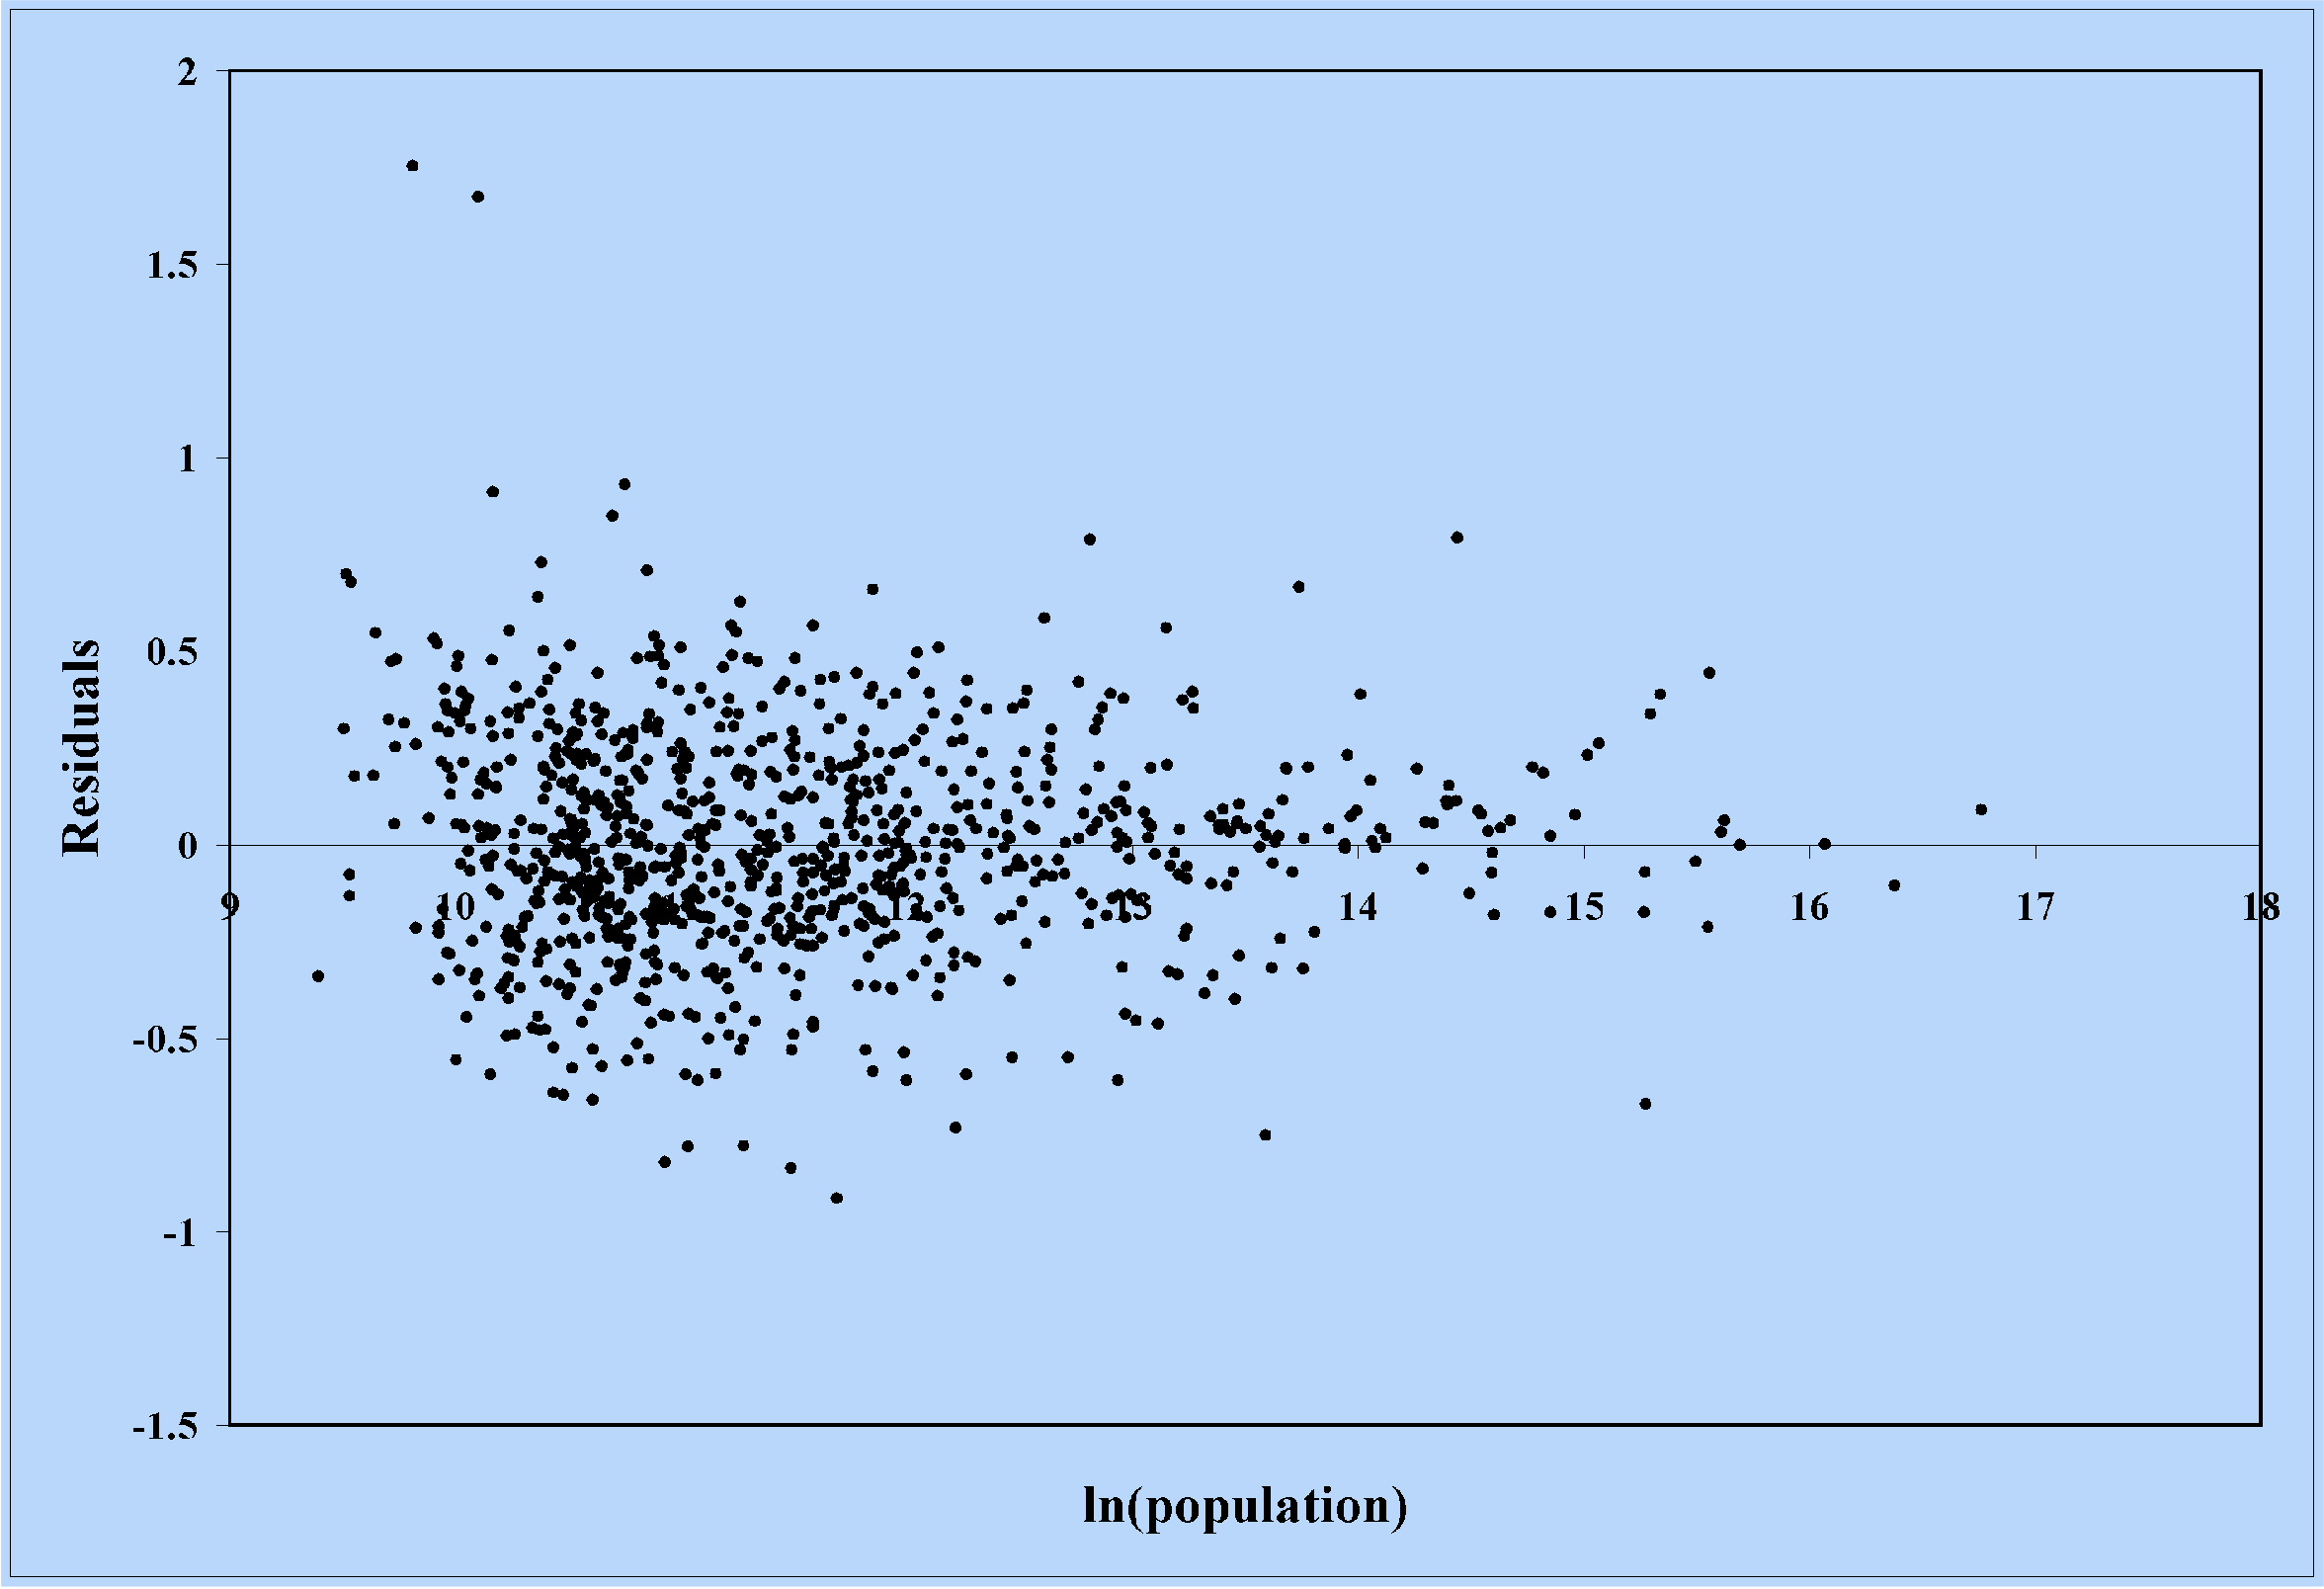
\includegraphics[scale=0.30]{fig/residuals-lobo.png}
\caption{Residuals from regressing ln(total wages) on ln(population) using data for all 943 urban areas of the United States showing larger unexplained components for smaller cities. \cite{loboUrbanScalingProduction2013}.}\label{fig-residuals-lobo}
\end{figure} 
These considerations lead us to consider the question: if financialization is redistributing the surplus generated by the growth of the urban system, could it also affect  productivity of the city itself, explaining a portion of the variation identified in the scaling literature? 



 %However, there is variation between regions that has not yet been adequately explained.
% {\newpage\thispagestyle{empty}
% \vspace{-1.5cm}
\begin{figure}[h!tb]
%\vspace{-1cm}
\begin{adjustwidth}{-0.24\textwidth}{-0.24\textwidth}
\centering
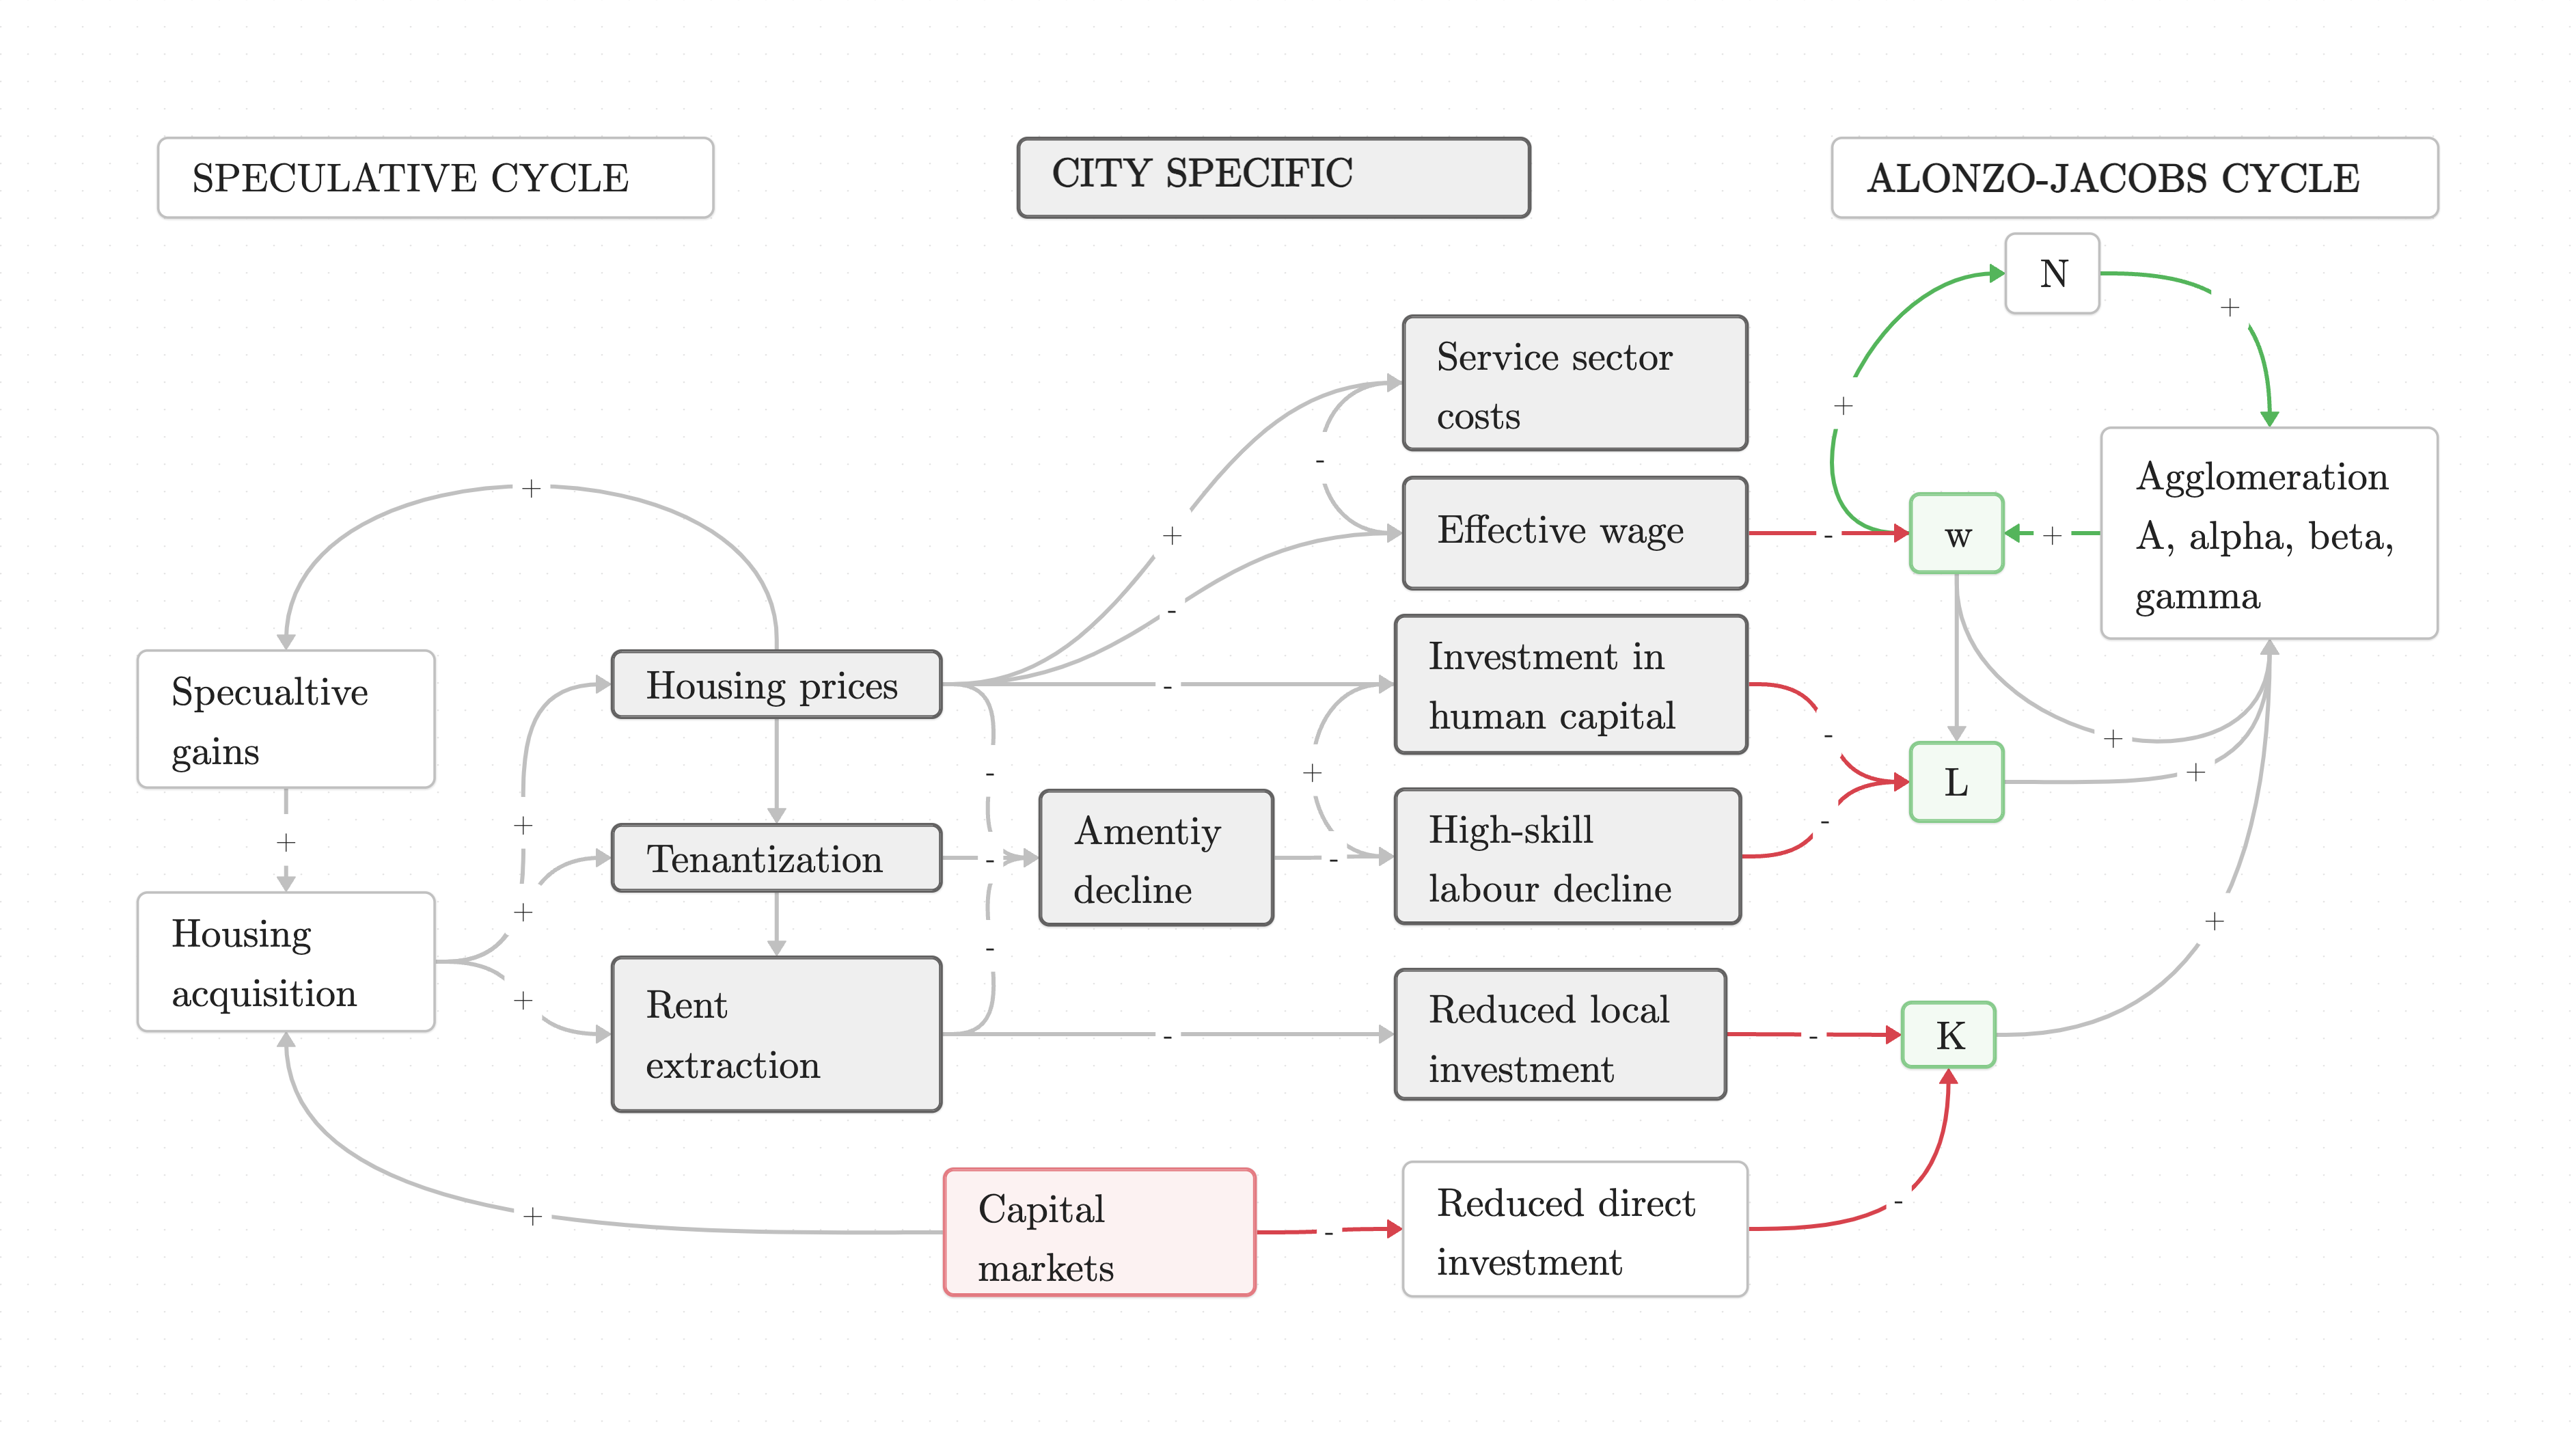
\includegraphics[scale=.15 ]{fig/impact-channels.png}%angle=90
\end{adjustwidth}
\caption{Impact channels relating financialization and urban productivity.} \label{fig-impact-channels}
\end{figure}
%}


\section{Channels through which financialization may affect productivity}

There are multiple and variable channels that %in theory 
might link financialization to the magnitude of agglomeration effects in different regions. Figure~\ref{fig-impact-channels} illustrates potential channels. %\footnote{The figure shows only some of the links and feedbacks. Each of the linkages shown or mentioned warrants extensive research, and for most even a brief literature search will reveal many related papers.} 
In the figure, the production sector is on the right, the processes occurring within the city are central, and the speculative intervention in the housing market is to the left. In the upper right, we show the \gls{Alonzo-Jacobs cycle}, described in Chapter~\ref{chapter-model}. In the Alonzo-Jacobs cycle, the strength of the agglomeration effect determines productivity, which in turn drives wages, which determines population which feeds back to agglomeration. In our model, anything that affects productivity must work through the parameters $A$, $\alpha$, $\beta$, or $\gamma$ or through factor supply. If any of the channels we describe below are significantly affected by financialization, governments may be able to increase social wealth and well-being through policy instruments at affect the level or impact of financialization. 

The fairly preliminary typology we present below, is intended to establish that links between financialization and productivity should be explored. We believe that the arguments in this section do establish the plausibility of linkages, but have found relatively little research on how financialization might affect productivity, % perhaps because researchers have not looked for links, 
so there is little explicit empirical work on the linkages to draw on. 
If there is any effect at all, however, it would be significant 
% The effect is particularly worth investigating 
since any negative effect on urban productivity can have significant consequences at the national level. Over 80\% of Canadians live in urban centres. Two-thirds of the economic growth in Canada was generated in its six biggest metropolitan areas and about 80\% of the growth comes from the urban areas in total \cite{w.fanImportanceCitiesEmphasis2010}. Simply calculating values, a reduction of 1.5\% in the productivity growth of these six large metropolitan areas alone would reduce the national growth rate by 1\%. Over 40 years the loss would be equivalent to 33\% of current GDP.

In this Chapter, we will describe the potential linkages between productivity and financialization and describe potential implementations for each linkage. In Chapter~\ref{chapter-results} on results, we implement a single aggregate linkage and show evidence from the model that the impact of these linkages would be substantial, suggesting that further research would be valuable.

%making it indistinguishable from the Jacobs model at the urban level. 
%In addition, the variation suggests that  financialization may have an impact through multiple channels.  

%{\color{red} In the next section we discuss potential linkages  with reference to the two dominant theoretical frameworks for understanding agglomeration effects, %. Second, it introduces the micro-foundations, the mechanisms by which agglomeration happens, drawing on the literature, and discussing how financialization might affect those mechanisms. Finally, in section~\ref{section-impact-channel-summary}, we summarize the primary linkages as they might appear in our model.} 

% {\color{red}WHAT IS AN IMPACT CHANNEL, WHY ARE WE ASKING THIS -- BY WHAT MEANS. FINACIALIZATION DOES THIS, PRODUCTIVITY IS THIS. THERE IS NOT NECESSARILY A CONNECTION, BUT THERE ARE CONNECTIONS. 
% Not one is dependant on another necessarily, but they are related in these ways.
% They are two distinct things that are not necesarily conected, but it does seem likely there i s an impact, so what are the channels. 

% Why are they seperate 
% urban productivity involves this feature this featuer this featuer
% financialization of the housing system has this feature this feature and this feature...

% MOST IMPORTANT THINGS

% ADD WHERE WERE GETTING THIS INFORMATION..- SAY WHAT THE SOURCES ARE..
% }

% The literature on financialization generally focuses on the housing market and the social consequences of rising home prices and tenantization.  Relatively few researchers discuss the several possible mechanisms by which financialization might affect the productivity of the city. 

% theory suggests a relationship that has not been observed, modelling can help identify the kind of evidend.%ANY THING OVERARCHING WE CAN SAY ABOUT THIS?LATER, IN CONCLUSION YOU SAY : To do this, we identified the housing market channels through which the changes in ownership might be transmitted through the economic and social body of of the city to the Alonso-Jacobs cycle, where agglomeration effects generate wealth.  

\subsection{Reduced capital stock}
Theorists have argued that financialization diverts capital investment from productive investment to financial enterprises \cite{lefebvreRevolutionUrbaine1970, harveyClassmonopolyRentFinance1974, harveyUrbanProcessCapitalism1978, christophersRevisitingUrbanizationCapital2011}. %The idea is that 
If more capital is diverted, it doesn't go into investments that increase the productivity of firms over time like equipment, facilities, etc. This direct reduction in \glspl{capital stock} % effect 
is illustrated at the bottom of Figure~\ref{fig-impact-channels}, where \glspl{capital market} can divert capital from the productive activities on the right to speculative activities on the left. Switching happens in response to the relative rates of return on the two sides. We have assumed a perfectly elastic supply of capital to firms and speculators. Extensions could model the effects of more complex and possibly more realistic capital markets. We allow the rate of return on housing investment to rise in response to city growth in the model, however, attracting speculative investment. We could also simulate a falling rate of return on non-housing investment by reducing the cost of capital to investors or by inhibiting the rate of growth of capital on the production side in response to rising investment in housing purchases. 


\subsection{Local investment}
Financialization may reduce the amount of local capital available, reducing investment in local activity. %raising the cost of borrowing money for certain activities in the city, which would make it harder to support the local economic activity. 
There are at least two mechanisms by which local investment capital may be affected. First, if increased tenantization and rent extraction reduce household wealth, we would expect household investment to decline. Second, this decline might be correlated with a decline in direct outside investment: when there is less money in a local economy, outside investors are less likely to see that economy as being as worthwhile an investment. This channel would act slowly and persist after an initial round of speculative activity as local housing is bought, and the money circulates in the economy. % and get counted in registers of local activity, encouraging further investment.

The second mechanism arises because taxing residents funds public infrastructure and services that are inputs to private production. Public inputs are usually ignored in the theory of the firm, but should not be ignored in the theory of the city.  The transportation network for example can usually be treated as an environmental constant, but transportation is a large sector and transportation costs may be a substantial share of firm costs. It is possible that with tenantization the city might face challenges in raising the tax revenue for spending on infrastructure, leading to a decline in overall productivity. The opposite might occur as well. Municipalities generally spend less on areas with tenants and collect more revenue per capita from rental housing, so tenantization might lead to more money available for % rising pressure for 
infrastructure expenditures. 

We could capture these effects by linking the owner-occupier ratio to the capital stock. We might also introduce a political market in which tenants and owners vote according to their own interests. Owners gain from property value increases, while tenants do not, giving them different incentives for voting at the municipal level. A more detailed approach might make the share of municipal taxes allocated to increasing agglomeration effects depend on a voting rule.


\subsection{High-skill labour decline}
Rising housing prices and a market dominated by rentals may make a city less attractive to highly skilled labour, making it more difficult to attract people with the specific adaptive skills needed for productive activities. %Glaeser and Saiz \cite{glaeserRiseSkilledCity2003} identified specific skills that tend to matter. 
Slowing in-migration or increasing out-migration of the more skilled members of the labour force will \textit{ceteris paribus} reduce the effective supply of labour. 
For example, Liu et al. \cite{liuImpactUrbanHousing2023} found for China that an increase in urban housing prices has a crowding-out effect on labour mobility.  Duffy et al.  \cite{duffyRisingHousePrices2005} found that for Ireland that rising house prices, by discouraging potential migrants, could significantly reduce the growth potential of the economy, shifting the balance of labour market growth from employment to wages, with a consequent deterioration in competitiveness. %Anecdotal evidence comes from comes form the frequent news stories about which cities are most livable: low housing prices are almost always an important element in the measures used. (we omit the link form  housing prices to high-skill labour. 

The reduction in highly skilled labour might be offset by importing human capital though immigration or raising wages for talent in the city. Florida\cite{floridaCompetingAgeTalent2005, floridaCreativeClassEconomic2014} has suggested that urban growth is strongly linked to the ability to attract talent. 
There is also a possible counter effect as some of the investment in financialized buy up of land may go towards improving neighbourhoods to attract higher rents.  
While \gls{tenantization} pushes skilled labour out of neighbourhoods, \gls{gentrification} can pull it in. Gentrification can be seen as trend opposing tenantization. Cornelissen and Jang-Trettien \cite{cornelissenHousingContextNeighborhood2023} point out that tenantization, neighborhood decline, and disinvestment are more common than gentrification in low-income neighborhoods and are likely to produce the opposite of the effects of gentrification. Althobaiti et al \cite{althobaitiHousingPricesSkills2021a} %%\cite{althobaitiHousingPricesSkills2021}  
show that with gentrification, high-skill workers % cognitive skills are getting 
move closer to the city center in response to the increase of median housing prices while low-skill physical skills moved further from the center.  

In the model, we could introduce this channel by making the labour elasticity of output in the Cobb-Douglas function, $\beta$, depend on the home-ownership ratio. High home ownership correlates with high income and high education, two factors that influence individual productivity. Individual productivity is represented by. $\beta$. %{\color{red} DESCRIBE EFFECT OF THIS RELATIONSHIP}


\subsection{The effective wage}
 Lobo et al. \cite{loboUrbanScalingProduction2013} find the \gls{effective wage} is one of the determinants of growth. The effective wage, also called the real wage is the wage corrected for changes in prices. If people have to pay more to live in the city at a given money wage as they do when rents rise, the effective wage has fallen. With a single sector as in our model, the level of wages and the level of rents are tightly linked. But what if some of the city population is producing services for the local population? That sector is unlikely to enjoy these same positive agglomeration effects as the export sector does when the population grows. Rising rents would lower the effective wage for workers in that sector. The cost of living rises for everyone but wages fall behind for service workers.  %have to become more expensive to cover the cost of labour. 
% that makes other goods and services more expensive.

%inflationary pressures may decrease the effective wage and 
In Figure~\ref{fig-impact-channels} we can see that inflation, coming from the right side of the diagram may reduce the effective urban wage, although we do not show sectoral effects. 
General financialization may also reduce the bargaining power of labor, as Tomaskovic-Devey and Lin argue \cite{tomaskovic-deveyFinancializationCausesInequality2013}, reducing wages.\footnote{Tomaskovic-Devey and Lin point to a shift in behaviour of non-finance firms away from production and non-financial services and toward financial investments and services. This shift, they argue, has led to lower employment, income transfers to executives and capital owners, and increased inequality among workers \cite{tomaskovic-deveyFinancializationCausesInequality2013}}
%In the second part of the chapter we implement several of the mechanisms and share results. 

Adding firms that produce for the local market or workers with different skills will allow us to investigate the effects of varying wages on different classes of workers. {\color{red} IDEALLY ADD ANOTHER SENTENCE OR TWO TO FILL OUT IMPLEMENTATION DESCRIPTION}

% VERY INTERESTING \cite{buchlerImpactHumanCapital2024} in areas with elastic housing supply, the positive demand shock leads to the construction of more housing, a larger labour force, and, thus, moderate wage growth. In contrast, in areas of low housing supply, the positive demand shock has a limited impact on new housing construction and the urban population. Human capital gets capitalised into higher home prices, hindering urban growth.


\subsection{The amenity channel}
Urban amenities are part of the incentive for choosing city life, and a decline in amenity will have a similar qualitative effect on productivity as a decrease in the wage.  If the effective wage of  baristas declines, for instance, the supply of labour to coffee shops should decline. To compensate, the wages of baristas would have to rise. Some caf\'es could close and others raise prices to cover the higher cost of labour. Closing businesses directly reduces, but both closures and higher prices affects the amenity of other residents. Reduced amenity might then reduce the concentration of educated personnel by % reducing the diversity and amenity of cities, 
making urban living less attractive, reducing labour supply, or raising its cost. 
On the other hand, if developers compete for a limited number of higher income residents, they may compete to raise amenity along with costs in some neighbourhoods. If there are higher rents, or a larger share of taxes from increased \gls{tenantization}, public investment in amenity could go up at least in the short term. % As with local local investment, if there are more taxes collected from tenants, there may be 

To explore the questions that arise with the introduction of amenity, we might introduce agents with different preferences and perhaps different skills. % If our concern includes the effects of different sectors, 
We might also explore the ways that amenity is produced---for instance though arts and entertainment, or the provision of things like parks and street maintenance by the city.
 

\subsection{Impact on the service sector}
Financialization may also have effects on the service sector that could feed back to affect productivity. The service sector is large. It makes up about two thirds to three quarters of the Canadian economy and includes transportation, education, healthcare, construction, banking, communications, retail services, tourism, other government services, and `non-material' activities or `intangible goods.' %It is not one industry---including 
The service sector includes everyone from the baristas mentioned above to real estate agents and university professors. 

Financialization might have a number of potential impacts on productivity via the service sector. To consider one example, rising housing costs at the centre of a city may push low-wage service workers to the edges, producing a spatial sort by income. We'd expect to see particular impact on the personal service sector. Pushing service workers to the edge of the city might also increase their transportation costs, putting further downward pressure on their effective wages while increasing the costs of those amenity services that rely on lower-cost workers, and thus reducing the amenity and effective wage for other workers in the city. 

We restrict our model to a single export industry in the base model. 
% Restricting our model to a single export industry is a clear limitation when we consider the potential effects of financialization. 
To explore the effect of financialization on the service sector, %this large and varied sector the model, 
we would need to  model specific subsectors. Because there are ages and income differences across the sectors we would also need to enrich our list of agent attributes. 


\subsection{Reduced investment in human capital}
%There is a vast literature on investment in human capital. 
Finally, there may be impacts on productivity through the reduction of human capital. 
% There are two major ways to grow a city's human capital. One is to 
It is possible to grow a city's \gls{human capital} by increasing how many workers there are, i.e. increase the labour supply, or by increasing their effectiveness by making workers more productive through training, education, etc. % the effective labour supply therefore grows faster than the labour supply as a result of increased education. 
This means investment in human capital can grow the \gls{effective labour supply} even without growing the total population.

Growth theory, discussed in Chapter~\ref{chapter-growth}, suggests that the growth of human capital is a major driver of productivity. Increasingly effective human capital increases returns to scale in the industrial sector and at the national level. 
Solaki \cite{solakiRelationshipEducationGDP2013} demonstrates a causal relationship between education and growth at the national level. Empirical results for Bangladesh \cite{islam2007relationship} show evidence of bidirectional causality between education and growth, which means that means if there's lower education, there's lower growth.  Among others, B\"uchler et al \cite{buchlerImpactHumanCapital2024} have recently confirmed the important of human capital growth for urban growth.
%Reduced local capital available for reinvestment in human capital might reduce the adaptive capacity of a city's population because people have reduced resources to buffer against challenges.
Rising productivity due to increasing human capital would raise wages. %  as we described in Chapter~\ref{chapter-growth} section~\ref{section-growth}.

There are at least two mechanisms by which investment in human capital may be affected by financialization. The most direct is by reducing household incomes. Increasing housing prices increases the wealth of owner-occupiers which may result in, for instance, increased spending on education for offspring.\footnote{On the other hand, increased housing costs for tenants may result in reduced human capital investment. Glaeser and Saiz found evidence for skill upgrading in declining cities, which suggested to them efficient investment in less skilled workers is a key adaptive/growth mechanism. If powerful enough, this effect might offset some of the negative impacts of financialization we have suggested.} %The effect may be different for different parts of the population. 
% In financialized markets, where more occupants are tenants as opposed to owners, this shift could have notable effects. 
% It is also possible that there are effects going the other way. For instance the signal from rising housing costs might trigger people to work additional hours or put rising shares of their income into competing in a more challenging environment, even if the total available to invest declines, the amount invested may go up if share increases sufficiently, as might be the case if there are a limited number of high paying or secure jobs.
Less directly, we suspect financialization will increase the cost of living through, for example, increasing labour costs in the service sector since it raises the cost of living and thus the wages people need to live in the city and work. Higher cost of living that may result in a reduction of the effective wage might also reduce income available for human capital investments. % Rent capture leading to 

We can simulate some human capital effects by making a link from the home-ownership ratio to the productivity parameters  $\beta$ and $A$. A more nuanced approach would be to introduce a training industry. %this has been done=

\section{Conclusion}
In this chapter, we have described a number of channels through which the effect of financialization is likely to affect productivity. % be transmitted to the Alonso-Jacobs cycle, where agglomeration effects generate wealth. 
Our list is not complete but it provides theoretical grounds for testing the model's sensitivity to a range of policy interventions and lays the foundation for empirical work.  

The dominant effect of financialization is to shift ownership of housing from occupiers to those who own financial capital. Understanding the mechanisms by which that might affect productivity has considerable policy importance because it raises the possibility that there are channels for public policy to enhance the positive effects of agglomeration. 

In  Chapter~\ref{chapter-model} we present a model in which we can systematically test the model's sensitivity to a range of policy interventions under the assumption that a link does exist. % if any spillovers to productivity of the type we discuss here exist. 
In the results section we will further explore, based on our analysis and simulations, how the % unrecognized 
impacts of financialization of the urban housing market may also have impact % extremely serious effects on 
the economy as a whole. Although determining the relative importance impact channels %in general or for a specific city 
is an empirical problem outside scope of this work, % the brief of this thesis but tests in the universe of the model can lay the foundation for later empirical work.  
the model can suggest directions for future work.

%Financialization may indirectly affect urban productivity at many points in the system. We defer extending the model to include these effects. Our focus in this chapter has been limited to examining possible channels through which the housing market financialization is likely to affect the productivity of a city. 

% We have modeled the relationship between ownership and the inputs to the aggregate production function described in Chapters~\ref{chapter-growth} and \ref{chapter-model}. 

% {\color{red}
% Essentially, the discussion in this chapter has guided and helps explain the policy experiments we have conducted. MAYBE ADD A FINAL SENTENCE PULLING IT ALL TOGETHER?}




% \subsection{TODO ADD BACK MOVE TO TRANSMISSION CHAPTER? The transmission puzzle}

% %The transmission of productivity increases arising from agglomeration effects  to the urban wage through firms, can be modelled in many ways. The agglomeration effects are external to the firm and therefore likely to be unexpected. If  firms underestimate the marginal product of labour, labour productivity will be greater than expected, output will be higher than planned output, and revenue and profits will therefore be higher than expected. Excess demand will attract more productive capital which in turn will demand more labour,  Rising labour demand drives up the wage. The agglomeration effect driving growth is essentially a public good in which individual firms will under-invest. This raises a policy challenge that we leave for others. CLARIFY -- ALSO STILL A FOOTNOTE IN MODEL SECTION. CUT OR REF THEiR IF MOVING HERE.

% % It is straightforward to compute the rate of excess return for  this model. 

% %
% \begin{figure}
% \centering
% 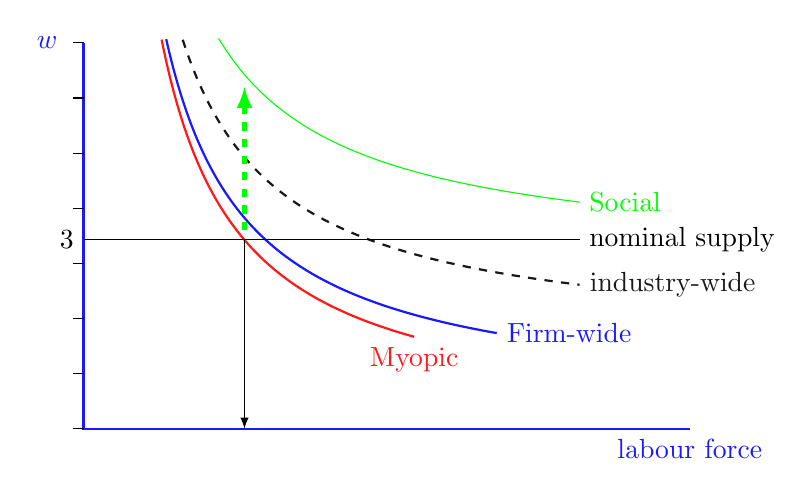
\begin{tikzpicture}[scale=.7]
%\def\bndmax{5}        %https://tex.stackexchange.com/questions/68462/filling-a-complex-region-with-tikz
%\def\bndmin{0.2}
\def \Y {7}  % height of y axis pecent
\def \W {15}  % length  of x axis
\def \Wbar {3} % jmeam wealth
\def \omega {3}
\def \A {1}  %was .5
\def \B {.5}

\draw [thick, color=blue!90] (0,\Y)node[left=.2cm]{$w$} -- (0,0)--(\W-4,0)node[below]{labour force};  
 \foreach \yi in {0,...,\Y} \draw (0,\yi)--(-.2,\yi)node[left]{};
 
\tikzset{func/.style={thick,  color=blue!90}}
% \draw[ func, domain=.2:\W-6] plot [samples=200] (\x, 2*\x^.5)node[below=.1, right]{SUPPLY};

\tikzset{func/.style={  color=green}}	
\draw[func, domain=2.45:\W-6] plot [samples=200] (\x, 10/\x+3)node[above=.1, right]{Social};

\tikzset{func/.style={thick, dashed, color=black!90}}	
\draw[func,domain=1.8:\W-6] plot [samples=200] (\x, 10/\x+1.5)node[ right]{industry-wide };

\tikzset{func/.style={thick, color=blue!90}}	
\draw[func,domain=1.5:\W-7.5] plot [samples=200] (\x, 10/\x+.4)node[below=.05, right]{Firm-wide};

\tikzset{func/.style={thick,color=red!90}}	
\draw[func,domain=8.5/6:\W-9] plot [samples=200] (\x, 10/\x)node[below]{Myopic};

\draw[](0,3.425)node[left]{$\omega$}--(9,3.425)node[right]{nominal supply };
\draw[thin,latex-](2.92,0)--(2.92,3.425); %a vertical labour supply
\draw[ultra thick,dashed, green,-latex](2.92,3.6)--(2.92,6.2);
%\draw [blue,  thick](13, 8.3)--(15,8.3)node [right, black] {\small A=\ 1,\ B=0.5};
%\draw [green, thick](13, 7.6)--(15,7.6)node [right, black] {\small A=.8, B=0.8};

%\node at (5,-1.5){Resulting in  profits, expansion, and/or entry: the city grows};
 \end{tikzpicture}
% \caption{Multiple marginal products.}
% \label{fig-multiple-marginal-products}
% \end{figure}



% %5Figure~\ref{fig-marginal-products} illustrates the problem. We can  make a distinction between the myopic marginal productivity curve observed  at the shop floor level and  the firm-wide effect of adding a worker. The red curve labeled ``Myopic'' represents the declining direct marginal productivity of labour as  might be observed by a shop manager, who could report how much more output one with one worker one lathe would produce. The blue line above it labeled ``Firm-wide'' represents the actual effect on firm productivity that arises because the new worker makes other workers in the firm more productive. This addition to output would be observable for managers reviewing the firm's performance over time. It might be most easily observed in small firms. 

% %We can go on to consider the slower and distributed effect on closely related firms, which would raise any estimate of marginal product.  If there are 10 other firms and a new worker  has a small spillover effect  $\epsilon$ on each,  the spillovers raise the industry  marginal product  by $10\epsilon$. Each of the  10 other firms  enjoys  an additional $10\epsilon$ gain in the marginal product of their workers. This should lead to additional hiring by other firms.

% %Finally, expanding our view another step, we notice that if each of the  10 other firms hires one worker who produces an additional  $10\epsilon$ gain in output for all firms, the total spillover effect would rise by $100\epsilon$. The social marginal product of a single hire is indicated by the green line. 


